\documentclass[output=paper]{langsci/langscibook.cls}
\ChapterDOI{10.5281/zenodo.1090988}
\title{Comparing novices and semi-pro\-fes\-sion\-als: False friends as a case in point}
\author{Iryna Kloster
\affiliation{FTSK Germersheim, Johannes-Gutenberg-Universtität Mainz}
}

\abstract{This publication presents interim results of a larger empirical study which aims at determining and measuring the differences between novice and semi-professional levels of competence. The study attempts to model translation competence, in particular to predict the level of competence based on empirical process data about the distribution of visual attention, revisions and the use of reference materials. In the study, collocations, idioms, realia and the like are used as stimuli. This contribution focuses on the reading and comprehension of false friends in the language combination Italian-German. False friends serve as the basis for contrasting translation performance of novices and semi-professionals. The participants were native speakers of German (L1), acquiring both language and translation competence in their L2 almost simultaneously. A combination of research methods was applied to collect process data within a series of experiments conducted at the Faculty of Translation Studies, Linguistics and Cultural Studies of the University of Mainz: eye tracking, keystroke logging, retrospective interviews and screen recording. The collected data were evaluated quantitively as well as qualitatively and then triangulated.}

% \textsf{\textbf{Key words:} }translation, competence, performance, false friends 

\begin{document}
\maketitle


\section{Theoretical framework}

This contribution focuses on the processing of false friends and looks at the differences between the two levels of competence -- novice and \isi{semi-professional}. Both groups of students had no or very little knowledge of their L2 prior to their translator training, that is, the acquisition of the language competence along with \isi{translation competence} played an essential role in developping their skills.  Foreign language acquisition based on the comparison of languages is still the dominant paradigm at the present time.  Contrastive analysis has aimed at the optimization of language didactics since the first attempts to compare languages \citep{Lado1957, Alatis1968, Fisiak1981}. The field departed from the belief that differences between languages cause difficulty in language learning \citep[10]{Hawkins1986}, therefore contrastive analysis was necessary to systematize the language structures, thus contributing to the improvement of learning materials.  According to \citet{PruferLeske1997}, contrastive analysis is given a major amount of attention in a traditional foreign language class in spite of the availability of a variety of other alternative methods of language acquisition. A prominent example of a translation-oriented contrastive and stylistic language analysis is that by \citet{Vinay1977}, with further studies in this direction being \citep{Truffaut1963, Henschelmann1980, Gallagher1982}, all of which attempted to solve translation problems by comparing language structures. Motivated by the fact that everyday translation practice requires practical techniques for frequent translation problems, including language contrasts, \citet{Konigs2011} pay particular attention to systemic language contrasts which may be relevant for translation.  Based on the findings of contrastive analysis, translators should be able to make conscious decisions and avoid solutions founded on pure intuition. Foreign language acquisition is also an important component of translator training according to the currently leading \isi{translation competence} models \citep{PACTE2000, PACTE2003, Gopferich2008, Gopferich2009Towards}
% \todo{Was PACTE1998, changed to PACTE2000 - is that OK?} 
in translation studies (a comprehensive overview of existing definitions and models of \isi{translation competence} is given in \citealt{Gopferich2008, Herold2010}).  Translation competence has interested researchers for decades: ``While for the uninformed, \isi{translation competence} often appears as the automatic by-product of second-language competence, translation scholars have known that there is more to translating than knowing two or more languages'' \citep[174]{Gopferich2009Process}. The existing empirical \isi{translation competence} models attempt to cover all possible multi-faceted fields of professional translators' activity and thus are versatile and rather complex. According to PACTE, the most important sub-competences that represent the essence of expert TC are \textit{strategic sub-competence}, \textit{knowledge about translation sub-competence} and \textit{instrumental sub-competence}. Undoubtedly, the field of a translator's profession extends far beyond the knowledge of the foreign language; however, the \textit{bilingual/linguistic} \textit{competence} remains one of its important constituent parts. After all, the evaluation of linguistic and \isi{translation competence} is an indispensable component of \isi{translation quality} assessment \citep[199]{Mertin2006}. According to PACTE, \textit{bilingual sub-competence} is ``pragmatic, socio-linguistic, textual and lexical-grammatical knowledge in each language'' \citep[610]{PACTE2005Investigating}. They assume the underlying knowledge behind the \textit{bilingual sub-}\textit{competence} to be for the most part procedural. \textit{Communicative competence} \textit{in at least two languages} in Göpferich's \isi{translation competence} model corresponds to PACTE's \textit{bilingual sub-competence}. ``Communicative competence in the \isi{source language} is relevant primarily 
for source-text reception, whereas target-language competence determines the quality of the target text produced'' \citep[21]{Gopferich2009Towards}. Another competence, which goes hand in hand with the \textit{bilingual/communicative sub-competence} and is the focus of interest in the present study, is the \textit{research competence}. PACTE calls it \textit{instrumental-professional competence} and subdivides it in two separate sub-competences: \textit{instrumental sub-competence} and \textit{knowledge about translation sub-competence}. The \textit{instrumental sub-competence} (mainly procedural knowledge) implies the usage of information, all kinds of documentation and communication technologies. The use of reference material is an indisputable part of a translator's work. The use of reference materials has been studied empirically by \citet{Krings1986Was, Jaaskelainen1989, Livbjerg2002}.

The \isi{translation competence} models mentioned above provide the theoretical environment for practical considerations, but they are not detailed enough to characterize the development of single sub-competences. A continuously growing number of empirical studies, which specifically compare the levels of competence, provide the definitions of sub-competences: professionals vs.\ non-profes\-sion\-als \citep{Breedveld2002, Jaaskelainen1999}; semi-professionals, professionals, young professionals, student translators \citep{Jarvella2002}; professional vs. student translators \citep{Carl2010Correlating}, and others. 

The way translators deal with language contrasts in the process of translation may shed light on the differences in translation expertise.  Despite the large number of studies on language contrasts, little research has been carried out on how translators approach language contrasts directly in the process of translation. One of the pioneer studies carried out by \citet{Jakobsen2007} was conducted using \isi{keystroke logging} as the method of data collection. The main purpose was to ``find evidence to help [the researchers] understand how idioms are processed by translators and interpreters'' \citep[217--218]{Jakobsen2007}.  \citet{Vandepitte2011} studied metonymic language in translation. Investigating to which extent metonymic language is a translation problem (= results in longer translation time) for translation students, they suspected the following: ``[\ldots] it is not clear to what extent cross-linguistic differences actually pose problems to most beginning translation students and therefore need a place in the training curriculum'' \citep[68]{Vandepitte2011}.  Their study confirmed their hypothesis, the results showing that ``it took translation students more time not only to translate metonymic constructions than their non-metonymic counterparts, but also to produce a non-metonymic \isi{construction} if the source text is metonymic than if it is non-metonymic'' \citep[127]{Vandepitte2015}.

This research project pursues similar goals regarding the processing of \textit{false friends}. False friends is a label usually applied to lexemes which are similar in both languages due to their phonological and orthographic form, but are different in meaning; at least one of the meanings in the \isi{target language} does not exist in the \isi{source language} \citep[295]{Pavlova2012}. Furthermore, ``~`false friend' [is] a word in one language which sounds like one in another and may be taken by mistake as having the same meaning.'' \citep[126]{Matthews2007}. 

False friends are a kind of cognate. Researchers distinguish between true and false cognates, but the distinction between true and false cognates can be fuzzy \citep{Taylor1976, Browne1982} in that \isi{cognate} pairs will often share some, but not all aspects of their meaning or use \citep{Perkins1985}; in certain contexts, they are true cognates, and in others false cognates \citep[174]{Shlesinger2005}.

\textit{False friends} are generally referred to as \textit{false cognates} and are a source of interferences on the word level for translators. False friends are therefore problematic for translators, as they seem, from a formal point of view, to be interlingually parallel, but are in fact not, because they have quite different meanings. When they encounter a \textit{false friend} in the process of translation, translators have two possibilities to deal with it: to prefer a \isi{target language} \isi{cognate} or to search for an alternative solution. Additionally, translators may avoid the usage of TL cognates on purpose and look for a creative solution. ``Given the positive values associated with creativity, one may expect the translator to be predisposed to search for the `more creative' solution, the `noncognate'{}'' \citep[176]{Shlesinger2005}. In their study ``Comparing modalities: cognates as a case in point'', Shlesinger and Malkiel investigate ``\isi{cognate} status, performance on false cognates, and \isi{cognate} processing'' based on target texts from translation and \isi{interpreting} \citep[176]{Shlesinger2005}. In the first part of the experiment, seven professional translators/interpreters interpreted a source text containing cognates from English into their native language and four years later they translated the same text once again. When presenting the results of their experiment, Shlesinger and Malkiel focused on true cognates and false cognates separately. They found that most of the true cognates appeared in their \isi{cognate} form both in \isi{interpreting} and translation. Nevertheless, it is worth mentioning that there were more noncognate solutions in translation than in \isi{interpreting}, possibly due to \isi{cognate} avoidance (c.f. also studies on monitoring and priming processes by de Groot and Oster in this volume). False cognates were translated correctly by means of noncognate alternatives in the vast majority of cases. In \isi{interpreting}, however, false cognates were more problematic presumably due to the ``minimax strategy'' \citep{Levy1967}, i.e. aiming at producing the most effect applying the least effort. 

\citet{Vintar2005} investigate shining-through and aversion in the use of cognates in \ili{German} and \ili{Slovene} translations of English. In their corpus study, they compare translated texts with originals in these languages to see whether there are differences between the use of cognates in translated and non-translated texts. Their analysis shows that the frequency of cognates in \ili{German} and \ili{Slovene} translations is similar. Further they found that \ili{Slovene} translations contain less cognates than the \ili{Slovene} originals, whereas \ili{German} translations include significantly more cognates than \ili{German} originals. Not only linguistic, but also cultural and political developments determine these results. While there is a strong influence of English on the \ili{German} language, the strengthening of the \ili{Slovene} national identity reinforces the purity of the language. 

\section{Hypotheses}

False friends are generally viewed as potentially problematic for translation. This assumption enables hypotheses about the way in which they are processed, i.e. read and perceived, by semi-professionals and \isi{novices}:  

\begin{enumerate}
 \item \isi{Novices} process false friends faster than semi-professionals while reading and comprehending the source text, i.e. \isi{total fixation duration} is shorter in the group of \isi{novices}.
 \item \isi{Novices} use the dictionary less frequently than semi-professionals.
\end{enumerate}


\section{Multi-method process based approach}

Contemporary research methods make it possible to combine/triangulate a number of research methods to study the \isi{translation process} and translators' performance simultaneously as well as to analyse a relatively large number of user activity data. A combination of methods was applied to gather data: eye tracking, \isi{keystroke logging}, retrospective interviews, screen recording and translation product evaluation. The instruments of data collection were the eye tracker Tobii TX300 and the \isi{keystroke logging} software Translog 2006. The structured retrospective interview used in this study provided individual information on the process of translation from the subjects' perspective. Eye tracking, \isi{keystroke logging} and screen recording bring researchers closer to what actually happens in the process of translation. 

\section{Participants}

Participants were for the most part students enrolled in a degree program of the Faculty of Translation Studies, Linguistics and Cultural Studies of the Mainz University in the summer semester of 2011. There were 28 participants in total. However, the data of 8 participants had to be excluded from data evaluation for different reasons (e.g. technical errors, loss of visual data). The definition of \textit{novice} and \textit{semi-professional} was carefully considered with regard to the participants' homogeneity (concerning the required level of skill and experience). Novices, here, are defined as students who possess the basic knowledge (after the completion of the \textit{basic course}\footnote{\textit{Basismodul}} of their curriculum) of \ili{Italian} and whose native language is \ili{German}. Furthermore, they meet the following requirements: 1) no or very little knowledge of \ili{Italian} prior to the start of their degree programme; 2) no or only short private trips to \ili{Italian}-speaking countries. 


Semi-professionals were defined as students in their final or pre-final semester before graduation. The first requirement applies equally to all of them, whereas long- or short-term stays in \ili{Italian} speaking countries were considered a positive but not obligatory factor for semi-professionals.


For translators, foreign language acquisition is typically the first phase in their education. This is particularly true for the so called \textit{beginner-level-L2}\footnote{\textit{Anfängersprachen}}, with no language knowledge required prior to beginning the study programme. The acquisition of \textit{beginner-level-L2} takes place during the course of the study programme, typically as part of a so called \textit{basic course}. Since novice and \isi{semi-professional} \isi{translation competence} levels are the main interest of this study, the important fact here is that participants did not have any knowledge of their foreign language (\ili{Italian}) prior to their translation education. The acquisition of basic language knowledge took place in the framework of the \textit{basic course} and through autonomous learning. Hönig describes the acquisition of the \textit{beginner-level-L2} in the following way: 


\begin{quote}
\textit{%
Erwerb der Grundkompetenz in einer Nicht-Schulsprache besteht vor allem in einer Anleitung zum Selbststudium. Das bedeutet: Die technischen Möglich\-kei\-ten von Sprachlabor und Videothek werden in einer Einführung dargestellt; das Lehrmaterial steht zum Selbststudium zur Verfügung. Der \textsf{''Fremdsprachenunterricht''} beschränkt sich auf eine Lenkung und Kontrolle dieses Selbststudiums. Es gibt keine Lehrveranstaltungen, in denen Syntax und Vokabeln gepaukt werden; die fremdsprachliche Grundkompetenz soll und muß der Studierende sich selbst aneignen. Die Aufgabe der Lehrperson besteht vor allem darin, den Lernfortschritt zu kontrollieren und nach Erreichung einer gewissen Grundkompetenz die Studierenden in die vorgesehenen Lehrveranstaltungen des Zentral-Moduls zu integrieren.
}\hfill\citep[167]{Honig1995}
\\\\
``The acquisition of the basic knowledge of a language which was not part of the school curriculum consists largely of instructions for autonomous learning.  That is, there is an introduction into technical possibilities of a language lab and a video library; the teaching materials are available for autonomous learning. The ``foreign language class'' is limited to direction and control of this kind of autonomous learning. There are no courses in which syntax and vocabulary are studied intensively; students must master the core skills of the foreign language on their own. The primary task of the tutor is to control the learning progress and to integrate students who achieve a certain level of competence into the \textit{courses of the central module.}''
\end{quote}


Certain characteristics of \textit{beginner-level-L2} make the investigation of the competence level rather difficult. \citet{PruferLeske1997} points out the lack of progress monitoring during language acquisition throughout the \textit{basic course}. In other words, the definition of a certain basic competence, which a novice should possess in order to start translating, remains questionable. Furthermore, the individual process of learning is not transparent enough for a translation student. Therefore, he or she is unable to consciously locate him-/herself on a progression scale.


In the case of \textit{beginner-level-L2}, the process of language acquisition takes place at the same time as the acquisition of \isi{translation competence}. It is not the goal of the present study to investigate and compare all the possible facets of \isi{translation competence} of \isi{novices} and semi-professionals. Instead, the study focuses on aspects of translators' performance during reading and comprehension, such as visual attention, dictionary usage and individual feedback regarding the difficulty of comprehension. 


\section{Experimental design}
\subsection{Experimental settings}

In the beginning of each individual appointment, participants were given some time to familiarize themselves with the eye lab environment. They were then informed about the conditions of the experiment and its structure, and were asked to fill out a questionnaire. The participants were informed about the skopos of the translation. There was no \isi{time pressure} during the translation task. After receiving the instructions, participants could view the Translog 2006 interface which had already been opened for them prior to receiving instructions. The original text was located in the upper part of the screen, the participants typed their translations in the lower part of the screen. The participants had one monolingual online dictionary by \textit{Corriere della Sera} at their disposal. \footnote{\url{http://dizionari.corriere.it/dizionario\_italiano/}} For dictionary consultations, participants were asked to use the Internet Explorer window which had been opened for them prior to the start of recording. To ensure a smooth \isi{translation process} without interruptions, interviews were conducted only at the end of each translation task (i.e. \textit{delayed retrospection} in terms of \citealt{Cohen1981}). However, in order to minimize loss of information and to overcome memory failure, participants could view the replay of their \isi{translation process} in Translog 2006, with both texts at their disposal: the original text and their translation. High validity of retrospective data can be achieved by combining the replay of the \isi{translation process} with the interview \citep[35]{Gopferich2008}. 

\subsection{Experimental texts}

The topics of the texts were fairly general due to the limited research opportunities and in order to keep the duration of \isi{translation process} relatively short (approximately 200 words). Furthermore, the topic of both texts is quite neutral: the first text deals with an innovation in the shape of a robot which helps out in hospitals and the second text discusses the influence of reading habits on the gross domestic product of Italy. Both texts are derived from Internet resources (see below), however, for practical reasons they were significantly manipulated. 


Due to practical considerations, the number of contrastive elements to be studied was limited to idioms, collocations, proper names, realia and false friends. Therefore, specific results could be filtered out from the vast amount of \isi{translation process} data obtained through the chosen methods of research. The decision to enrich the experimental texts with the aforementioned contrastive elements was reviewed critically by translation lecturers of the Faculty. However, these language contrasts have already been the focus of interest in past studies. 

\section{Instruments of data elicitation}

Since the amount of data collected in the course of a multi-method approach is vast, there is a need to identify relevant metrics (\tabref{kloster:tab:1}) in order to conduct an analysis. Total \isi{fixation duration} and total \isi{fixation count} are metrics which characterize the amount of visual attention. The connection between fixations and cognitive activity is based on the eye-mind hypothesis of \citet{Just1980}. Its core assumption is that eye movements and pupil dilation correlate with perceptual and cognitive processes \citep[173]{Gopferich2009Process}. In this study, \isi{total fixation duration} stands for the cognitive processing of one particular area of interest (AOI). In order to measure \isi{total fixation duration} throughout the process of translation, every stimulus was marked with the AOI-tool of the eye-tracker software to ensure the calculation of the total time spent fixating each particular AOI (TFD) and additionally the total number of fixations (TFC) inside an AOI (\tabref{kloster:tab:1}). 

\begin{table}
 \caption{Metric units, abbreviations and measuring units}
 \label{kloster:tab:1}
\begin{tabularx}{\textwidth}{Qll}
\lsptoprule
Metric & Category & Measuring unit \\
\midrule
Total \isi{fixation duration} (TFD) & Reception metric & s \\
Total \isi{fixation count} (TFC) & Reception metric & times \\
Dictionary consultations (DIC) & Reception metric & times \\
Product evaluation (PRE) & Production metric & \isi{cognate}\slash non-cog\-nate\slash erroneous \\
Individual comprehension evaluation (ICA) & Reception metric & rating scale: -2 -- +2 \\
\lspbottomrule
\end{tabularx}
\end{table}



Dictionary consultations (DIC) is a metric representing the number of dictionary consultations related to a particular stimulus. The metric data was gathered manually by reviewing the screen recordings of the \isi{translation process}. 

\newpage 
Besides registering the length and number of fixations and the number and kind of dictionary consultations, participants in this study were asked to evaluate the comprehension difficulty of every language contrast. Individual comprehension evaluation (ICA) was based on a rating scale from 0 to 3 (0: very easy, 1: easy, 2: difficult, 3: very difficult) with no middle value. ICA values are expected to reflect the conscious individual assessment of comprehension complexity. 

Product evaluation (PRE) is a metric unit evaluating the \isi{acceptability} of the translation product.



\section{Results}

\subsection{General data} 

Before focusing on false friends, it is worth taking a look at the general data of the translation sessions of both groups of students. \tabref{kloster:tab:2} shows that the duration of translation (``initial orientation'', ``drafting'' and ``\isi{revision}'', \citealt{Jakobsen2002Orientation}) is, on average, longer in the group of \isi{novices}. This is not surprising as novice translators are generally known to be slower than professional translators. A closer, separate look at the source and the target text reveals some further information about the visual attention of both groups of participants. While \isi{novices} fixate the source text longer than semi-professionals, the amount of visual attention on the target text is quite similar in both groups. When we compare the \isi{total fixation duration} of the source and target texts in general, we come to the conclusion that semi-professionals are more busy producing the target text (15\% and 24\% more time spent on target \isi{text production} than on source text comprehension) and \isi{novices} comprehending the source text (sligtly over 20\% more time spent on source text than on the target text). The values of the total \isi{fixation count} confirm this assumption, demonstrating that \isi{novices} look quite more often at the source than at the target text. 

\begin{table} 
\small
 \caption{General data (T1-text 1; T2-text 2)}
 \label{kloster:tab:2}
\fittable{
\begin{tabular}{l r@{\,}r r@{\,}r r@{\,}r r@{\,}r r@{\,}r r@{\,}r@{\,}}
\lsptoprule
 & 
\multicolumn{2}{p{1.5cm}}{\centering Translation time (s)} &
\multicolumn{2}{p{1.5cm}}{\centering TFD ST (s)} & 
\multicolumn{2}{p{1.5cm}}{\centering TFD TT (s)} & 
\multicolumn{2}{p{1.5cm}}{\centering TFC ST (times)} & 
\multicolumn{2}{p{1.5cm}}{\centering TFC TT (times)} & 
\multicolumn{2}{p{1.0cm}}{\centering DIC (times)} \\
%  \midrule
& \multicolumn{1}{c}{T1} & \multicolumn{1}{c}{T2} & \multicolumn{1}{c}{T1} & \multicolumn{1}{c}{T2} & \multicolumn{1}{c}{T1} & \multicolumn{1}{c}{T2} & \multicolumn{1}{c}{T1} & \multicolumn{1}{c}{T2} & \multicolumn{1}{c}{T1} & \multicolumn{1}{c}{T2} & \multicolumn{1}{c}{T1} & \multicolumn{1}{c}{T2}  \\
\midrule
Mean (nov) & 2347 & 1477 & 444.9 & 685.0 & 343.0 & 533.7 & 1346.7 & 1904 & 907.8 & 1562 & 15 & 26.5  \\
Mean (semi) & 1475 & 1116 & 305.1 & 410.5 & 357.1 & 539.4 & 1084.0 & 1360 & 980.4 & 1454 & 7 & 1.0  \\
\lspbottomrule
\end{tabular}
}
\end{table}


\newpage 
Throughout the \isi{translation process}, \isi{novices} made use of the dictionary much more often than semi-professionals. This kind of discrepancy is not surprising, because \isi{novices}' vocabulary in their \textit{beginner-level-L2} is expected to be in the active stage of development. 

\subsection{Product evaluation} 
The meaning of the \textit{false friends} selected for the present study depends largely on their context. In certain contexts \textit{fenomeno (FEN)}, \textit{mito (MIT)}, \textit{idolo (IDO)} and \textit{fiction (FIC)} can be translated as true cognates, i.e. as \textit{Phänomen}, \textit{Mythos}, \textit{Idol} and \textit{Fiktion}. However, in the context of the experimental texts they behave as false cognates.  The results of the evaluation show that suitable solutions for \textit{fenomeno} were \textit{Neuheit}, \textit{technische} \textit{Errungenschaft} or verbal constructions, such as \textit{Ärzte} \textit{und} \textit{Patienten} \textit{sind} \textit{begeistert}; good solutions for \textit{mito} were \textit{unglaublich}, \textit{ein} \textit{Wunder};  \textit{idolo} was successfully translated as \textit{Liebling} or \textit{Vorbild}, whereas the most suitable solution for \textit{fiction} was \textit{Serie} or \textit{TV}{}-\textit{Serie}.  As for the overall classification of translation solutions, they were subdivided into non-\isi{cognate} (=acceptable), \isi{cognate} (=not acceptable) and others (=omissions and other erroneous solutions). The final evaluation of the translation product shows, that the relation between \isi{cognate} and non-\isi{cognate} solutions in the group of \isi{novices} is 21 to 16, whereas in the group of semi-professionals it is 8 to 26. These results complement the distribution of reception and production difficulties encountered by participants (\figref{kloster:fig:4}),  making it transparent that \isi{novices} largely consider false friends as a simple task, whereas the awareness of their tricky nature grows with the development of the \isi{translation competence}. 

\begin{figure}
    \begin{tikzpicture}
        \begin{axis}[
            width  = \textwidth,
            height = .3\textheight,
            ylabel={Amount},
            xlabel={}, 
            symbolic x coords={cognate solution, non-cognate solution, not acceptable},
            xtick=data,
            axis lines*=left,  
            ymin=0,
            ybar,
            bar width = 18pt,
            nodes near coords,
            nodes near coords align={vertical},
            axis on top,
            ymajorgrids, tick align=inside,
            major grid style={draw=white},
            enlarge x limits=true, 
        ]    
        \addplot+[lsMidBlue!80!black,fill=lsMidBlue] coordinates {(cognate solution,21) (non-cognate solution,16) (not acceptable,3)};
        \addplot+[lsMidOrange!80!black,fill=lsMidOrange] coordinates {(cognate solution,8) (non-cognate solution,26) (not acceptable,2)};
        \legend{nov, semi}
        \end{axis}
    \end{tikzpicture}
    %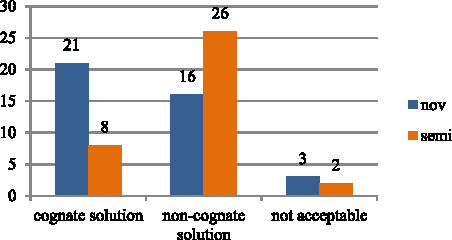
\includegraphics[width=.5\textwidth]{figures/kloster/figure1.pdf}
    \caption{Product analysis}
    \label{kloster:fig:1}
\end{figure}

\subsection{False friends: analysis of visual data}
The mean values of the \isi{total fixation duration} (\figref{kloster:fig:2}) show that both groups devote nearly the same amount of visual attention to false friends throughout the process of translation: the difference between the groups ranges merely from 0.1 ms to 1.9 ms. The hypothesized difference between \isi{novices}, namely that they adopt false friends automatically, and semi professionals, who are presumed to consider alternatives which would suit the context, is not given. The mean value of the total \isi{fixation count} (\figref{kloster:fig:3}) does not show any spikes either. However, the \isi{fixation count} data show that \isi{novices} fixate false friends slightly more frequently than semi-professionals which demonstrates that they reread parts of the source text several times.  

\begin{figure}
    \begin{tikzpicture}
        \begin{axis}[
            width  = \textwidth,
            height = .3\textheight,
            ylabel={},
            xlabel={}, 
            symbolic x coords={FEN, FIC, IDO, MIT},
            xtick=data,
            axis lines*=left,  
            ymin=0,
            ybar,
            bar width = 18pt,
            nodes near coords,
            nodes near coords align={vertical},
            axis on top,
            ymajorgrids, tick align=inside,
            major grid style={draw=white},
            enlarge x limits=true, 
        ]    
        \addplot+[lsMidBlue!80!black,fill=lsMidBlue] coordinates {(FEN,2.0) (FIC,5.5) (IDO,6.0) (MIT,4.0)};
        \addplot+[lsMidOrange!80!black,fill=lsMidOrange] coordinates {(FEN,2.2) (FIC,4.4) (IDO,6.1) (MIT,2.1)};
        \legend{nov, semi}
        \end{axis}
    \end{tikzpicture}
    %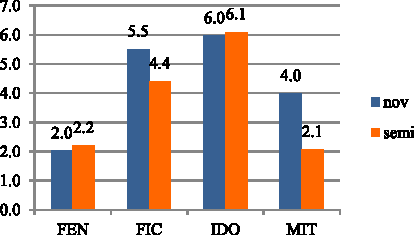
\includegraphics[width=.5\textwidth]{figures/kloster/figure2.pdf}
    \caption{Total fixation duration (mean/ms)}
    \label{kloster:fig:2}
\end{figure}

\begin{figure}
    \begin{tikzpicture}
        \begin{axis}[
            width  = \textwidth,
            height = .3\textheight,
            ylabel={},
            xlabel={}, 
            symbolic x coords={FEN, FIC, IDO, MIT},
            xtick=data,
            axis lines*=left,  
            ymin=0,
            ybar,
            bar width = 18pt,
            nodes near coords,
            nodes near coords align={vertical},
            axis on top,
            ymajorgrids, tick align=inside,
            major grid style={draw=white},
            enlarge x limits=true, 
        ]    
        \addplot+[lsMidBlue!80!black,fill=lsMidBlue] coordinates {(FEN,10.3) (FIC,15.2) (IDO,13.3) (MIT,9.3)};
        \addplot+[lsMidOrange!80!black,fill=lsMidOrange] coordinates {(FEN,8.7) (FIC,14.3) (IDO,12.9) (MIT,7.7)};
        \legend{nov, semi}
        \end{axis}
    \end{tikzpicture}
    %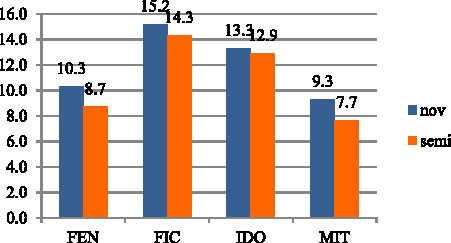
\includegraphics[width=.5\textwidth]{figures/kloster/figure3.pdf}
    \caption{Total fixation count}
    \label{kloster:fig:3}
\end{figure}


\newpage 
We can assume that visual parameters show a very similar \isi{cognitive load} in the processing of false friends by both groups of participants. Behind these values, the retrospective verbal data reveal that the distribution of difficulties encountered by both groups is not quite the same. 


\figref{kloster:fig:4} shows that in 25/40 cases, semi-professionals encounter production difficulties and in 6/40 cases, reception and production problems. 


\begin{figure}
    \begin{tikzpicture}
        \begin{axis}[
            width  = .75\textwidth,
            height = .4\textheight,
            ylabel={},
            xlabel={}, 
            symbolic y coords={reception, reception and production, production, no difficulties},
            ytick=data,
            axis lines*=left,  
            xmin=0,
            xbar,
            bar width = 12pt,
            nodes near coords,
            nodes near coords align={horizontal},
            axis on top,
            xmajorgrids, tick align=inside,
            major grid style={draw=white},
            %enlargelimits=true,
            enlarge y limits  = 0.2, 
        ]    
        \addplot+[lsMidBlue!80!black,fill=lsMidBlue] coordinates {(9,reception) (6,reception and production) (25,production) (0,no difficulties)};
        \addplot+[lsMidOrange!80!black,fill=lsMidOrange] coordinates {(8,reception) (11,reception and production) (11,production) (0,no difficulties)};
        \legend{nov, semi}
        \end{axis}
    \end{tikzpicture}
    %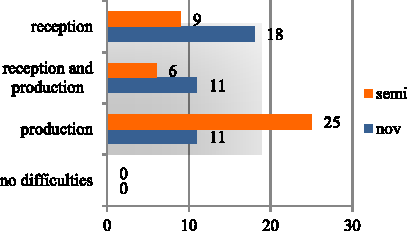
\includegraphics[width=.5\textwidth]{figures/kloster/figure4.pdf}
    \caption{Difficulties in reception and  production}
 \label{kloster:fig:4}
\end{figure}


 
In a large number of cases, \isi{novices}, as expected, are not aware of the particularities of false friends within the given context and report twice as many (18/40) no-problem cases than the group of semi-professionals (9/40). The absence of difficulties in both groups has different reasons.

The majority of the \isi{novices} demonstrate their unawareness of the specific false friends difficulties by reporting no problematic cases. Participant P20 believes that \textit{Phänomen} is merely the \ili{German} equivalent of the italian \textit{fenomeno}:  \textsf{<(wie haben sie das wort fenomeno verstanden?) äm als phänomen also (-{}-) als halt was ganz besonderes so (hatten sie schwierigkeiten bei der übersetzung?) nee ich hab's einfach (.) das} \textsf{deutsche äquivalent genommen> (P20/nov -} \textsf{\textit{fenomeno -} PRE: Phänomen)}


\textsf{\textit{<(how did you understand the word fenomeno?) as phenomenon well (-{}-) as something very special (did you encounter difficulties during translation?) no i simply (.) took the german equival}\textit{ent> (}\textit{P20/nov -} \textit{fenomeno -} \textit{PRE: Phä}\textit{nomen)}}

\newpage 
Participant P06 has more than one translation solution for \textit{idolo}, however \textit{Idol} remains his favorite. It seems to express the meaning in the best way: \textsf{<(wie haben sie das wort idolo verstanden?) hm: ido:l (-) beziehungsweise einfach held wäre viel also (.) das idol (hatten sie schwierigkeiten?) nein> (P06/nov - idolo - PRE: Idol)}


<(how did you understand the word idolo?) hm: ido:l (-) or simply hero would be too much well (.) the idol (was it difficult to translate?) no> (P06/nov - idolo - PRE: Idol). 


Participant P21 relies upon the common but rather vague general definition of \textit{fiction}, not attempting to adapt it to the target context: \textsf{<(ist ihnen das wort fiction geläufig?) ja (hatten sie schwierigkeiten bei der} \textsf{übersetzung?) nein> (P21/nov - fiction - PRE: Fiction)}


<(is the word fiction familiar to you?) yes (was it difficult to translate?) no> (P21/nov - fiction - PRE: Fiction).


Semi-professionals counteract the difficulties with their awareness of the specificities of false friends' specificity and are cautious translating them into \ili{German}. The following examples also show that semi- professionals are more wordy in defending their solutions than \isi{novices}: \textsf{<(wie haben sie das wort mito verstanden?) ach so semplicemente un mito ich hab das alle schon gelesen (-) ein wunder habe ich gesagt (-) mythos habe ich auch nicht mehr nachgeguckt im wörterbuch (.) bin gleich auf wunder gegangen (-) weil es etwas außergewöhnliches ist} \textsf{(würden sie hier mythos reinschreiben?) [nein (wieso?) mythos ist für mich was (-) nicht so real und der ist ja DA und das ist ein wunder (-) dass es funktioniert (hatten sie schwierigkeiten bei der übersetzung?) nein> (P25/semi -} \textsf{mito -} \textsf{PRE: Wunder); <(wie haben sie das wort idolo verstanden?) ja (-) so wie der traum oder das (-) auf was die ärzte eben gewartet haben (hätten sie andere vorschläge für idolo) (...) [ne> (P28/semi -} \textsf{idolo -} \textsf{PRE: der Traum).}


\textsf{\textit{<(}\textit{how did you understand the word mito?) o well} \textit{semplicemente un mito} \textit{i have already read it} \textit{(-)} \textit{i said a wonder} \textit{(-)} \textit{i haven't looked up myth} \textit{in the dictionary any more} (.) \textit{i picked wonder right away} \textit{(-)} \textit{because it is something very unusual} (\textit{would you also accept myth as solution}\textit{?) [}\textit{no} (\textit{why}?) \textit{myth is something} \textit{(-)} \textit{not as real} \textit{and THIS ONE it is kind of a wonder} \textit{(-)} \textit{tha}\textit{t it} \textit{functions} (\textit{did you encounter difficulties during translation}?) \textit{no}\textit{> (P25/semi - mito - PRE: Wunder); <(}\textit{how did you understand the word idolo}?) \textit{yes} \textit{(-)} \textit{something like a dream or so} \textit{(-)} \textit{what the doctors were waiting for} (\textit{any other solutions for idolo}\textit{) (...)} [\textit{no}\textit{> (P28/semi - idolo - PRE: der Traum).} }

When they integrate false friends into the target context, semi-professionals often pick creative solutions like \textit{der ... Vorbildcharacter hat} or \textit{Vorbild} for \textit{idolo}; \textit{phänomenaler Erfolgszug} for \textit{fenomeno}, which explains the time consuming procedure of producing a translation. A relatively small number of cases in the category false friends caused both reception and production difficulties within both groups (11 nov/6 semi). As opposed to participants who merely report production difficulties because they are familiar with the meaning of false friends in the source text, some participants are uncomfortable with the ambiguity of false friends in the \ili{Italian} source texts, which remains an obstacle on the way to a translation solution. Participant P01 declares that he is familiar with the word \textit{fiction} in the English language, but becomes a challenge in the present context: <(ist \textsf{Ihnen das Wort fiction geläufig?) aus dem englischen schon aber in dieser genauen wortbedeutung in bezug aufs fernsehen (-{}-) nicht (...) ja (.) ich weiß auch nicht genau ob ich das richtig getroffen habe > (P01/semi -} \textsf{\textit{fiction -} PRE: neue Fernsehreihe)}

\textsf{\textit{<(}\textit{is the word fiction familiar to you}?) \textit{sure from English but this particular meaning related to television} \textit{(-{}-)} \textit{not (...) yes} (.) \textit{I don't even know exactly if I got it right} \textit{> (P01/semi - fiction - PRE: neue Fernsehreihe).} }Participant P26 reflects upon the semantics of \textit{mito} in the source and the target languages and deducts the concrete meaning from the general idea: \textsf{<(...) ich weiß es nicht (-) ob es jetzt diesen roboter wirklich gibt oder nicht weil mythos ist etwas (-) wovon man nicht sicher ist ob es wirklich gibt oder gegeben hat oder nicht und das kann ich einfach nicht einfach so schreiben (-) wenn ich gar nicht weiß (-) ob er wirklich entwickelt wurde und es den gibt kann ich ja nicht nicht sagen (-) er ist ein mythos> (P26/semi -} \textsf{\textit{mito -} PRE: wie ein Märchen!)} 


<(...) I don't know if this robot really exists or not because myth is something (-) that you are not sure of whether it really exists or has ever existed before or not and I can not simply write it down in this way (-) if I don't know (-) whether it has ever been developed and it exists I can't say that (-) it is a myth> (P26/semi - mito - PRE: wie ein Märchen!)

In order to systematize sporadic comments, typifying them according to their central idea has proved useful. Some participants from both groups compensate for their reception difficulties with the influence of their previous knowledge about \textit{fenomeno, fiction, mito} or \textit{idolo} from other languages, for example English. It is firmly embedded into the procedural knowledge of participants and is the starting point for translation. The next reception problem is motivated by the unfamiliarity within the given context. Participants seem to know the concept behind the case, but cannot localize it in the given source text. In a situation where the translator is aware of the fact that hundred percent reception is not guaranteed, but the translation is expected to be provided, \isi{novices} turn to the target text and look for a solution which is acceptable but not idiomatic. 

The general evaluation of the quality of reported difficulties (\figref{kloster:fig:5}) demonstrates that, for the most part, they refer to \isi{translation competence} of participants. Finally, it should be mentioned that participants mostly remained dissatisfied with their translation solutions. 

\begin{figure}
    \resizebox{\linewidth}{!}{
        \def\pieangle{0}
        \def\pieradius{3}
        \def\piecyclelist{{"lsMidOrange","lsMidBlue","lsLightBlue"}}
        \newcount\piecyclecount \piecyclecount=-1
        \newcount\pieind \pieind=-1
        \begin{tikzpicture}
            \foreach \percent/\name in {
                58/semi: \isi{translation competence} (31),
                35/nov: \isi{translation competence} (19),
                7/nov: language competence (7),
            } {
                \ifx\percent\empty\else             
                    \global\advance\piecyclecount by 1     
                    \global\advance\pieind by 1            
                    \ifnum3<\piecyclecount                 
                        \global\piecyclecount=0              
                        \global\pieind=0                     
                    \fi
                    \pgfmathparse{\piecyclelist[\the\pieind]} 
                    \edef\color{\pgfmathresult}        
                    \draw[fill={\color},draw={\color}] (0,0) -- (\pieangle:\pieradius) arc (\pieangle:\pieangle+\percent*3.6:\pieradius) -- cycle;
                    \node at (\pieangle+0.5*\percent*3.6:0.7*\pieradius) {\percent\,\%};
                    \node[pin=\pieangle+0.5*\percent*3.6:\name] at (\pieangle+0.5*\percent*3.6:\pieradius) {};
                    \pgfmathparse{\pieangle+\percent*3.6} 
                    \xdef\pieangle{\pgfmathresult}
                \fi
            };
        \end{tikzpicture}
    }
    %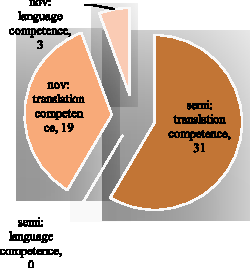
\includegraphics[width=.5\textwidth]{figures/kloster/figure5.pdf}
    \caption{Quality of difficulties}
    \label{kloster:fig:5}
\end{figure}


\subsection{False friends: dictionary consultations} 
The monolingual dictionary was used in both groups by some participants to look up the false friends, but in most cases the number of lookups did not exceed one (\figref{kloster:fig:6}). Only \textit{fenomeno} was not looked up, presumably because it is used much more frequently in the spoken language than the other false friends in the experimental texts. Looking at the temporal distribution of dictionary consultations over the course of the \isi{translation process}, the majority of participants made use of it during the \isi{drafting phase}: after having read the sentence containing a false friend and -- before translating it -- they opened the dictionary window (\figref{kloster:fig:7}). 

\begin{figure}
	\begin{tikzpicture}
        \begin{axis}[
            width  = \textwidth,
            height = .4\textheight,
            ylabel={},
            xlabel={}, 
            symbolic y coords={dic.fen, dic.fic, dic.mit, dic.ido},
            ytick=data,
           	axis lines*=left,  
        	xmin=0,
            bar width = 12pt,
        	xbar,
        	nodes near coords,
            nodes near coords align={horizontal},
           	axis on top,
        	xmajorgrids, tick align=inside,
        	major grid style={draw=white},
        	%enlargelimits=true,
            enlarge y limits  = 0.2, 
        ]    
        \addplot+[lsMidBlue!80!black,fill=lsMidBlue] coordinates {(0.00,dic.fen) (0.6,dic.fic) (0.7,dic.mit) (0.5,dic.ido)};
        \addplot+[lsMidOrange!80!black,fill=lsMidOrange] coordinates {(0,dic.fen) (0.6,dic.fic) (0.6,dic.mit) (0.6,dic.ido)};
        \legend{nov, semi}
        \end{axis}
    \end{tikzpicture}

 	%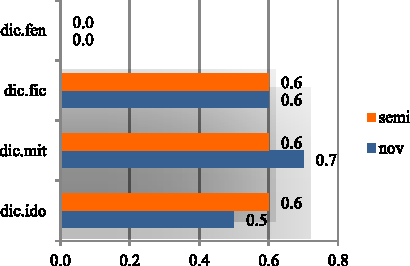
\includegraphics[width=.5\textwidth]{figures/kloster/figure6.pdf}
 	\caption{Dictionary consultations (mean/times)}
 	\label{kloster:fig:6}
\end{figure}

\begin{figure}
    \begin{tikzpicture}
        \begin{axis}[
            width  = 11.8cm,
            height = .3\textheight,
            ylabel={},
            xlabel={}, 
            symbolic y coords={after, immediately, before},
            ytick=data,
           	axis lines*=left,  
        	xmin=0,
        	xbar,
            bar width = 12pt,
        	nodes near coords,
            nodes near coords align={horizontal},
           	axis on top,
        	xmajorgrids, tick align=inside,
        	major grid style={draw=white},
        	%enlargelimits=true, 
            enlarge y limits  = 0.2,
        ]    
        \addplot+[lsMidBlue!80!black,fill=lsMidBlue] coordinates {(0,before) (12,immediately) (3,after)};
        \addplot+[lsMidOrange!80!black,fill=lsMidOrange] coordinates {(1,before) (13,immediately) (1,after)};
        \legend{nov, semi}
        \end{axis}
    \end{tikzpicture}
 %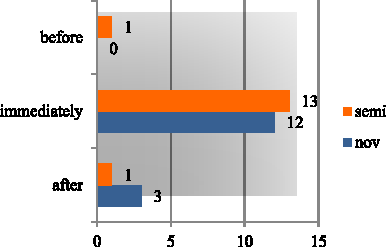
\includegraphics[width=.5\textwidth]{figures/kloster/figure7.pdf}
 \caption{Temporal distribution of dictionary look-ups}
 \label{kloster:fig:7}
\end{figure}

Some referred to the dictionary immediately, others reread the ST sentence several times (from two to five) before proceeding to the dictionary. Three \isi{novices} and one \isi{semi-professional} used the dictionary after having written down the translation. Two of the novice participants undertook changes in their solutions after the consultation: \textsf{<Vorbild $\rightarrow$ Held> (mito)} and \textsf{<ein Idol $\rightarrow$ das Idol> (idolo).} Only one semi- professional made use of the dictionary in advance: he read the whole passage, but did not start to translate it, instead he first read through the dictionary entries. After this dictionary session, he returned to the translation of the passage from the beginning. 

\newpage
The thoroughness of dictionary lookups was very individual. \figref{kloster:fig:8} shows that 10 \isi{novices} and 7 semi-professionals either did not read anything in the dictionary or stopped reading after the first line. 

\begin{figure}
    \begin{tikzpicture}
        \begin{axis}[
            width  = 11cm,
            height = .23\textheight,
            ylabel={},
            xlabel={}, 
            symbolic y coords={good -- complete, no -- little},
            ytick=data,
           	axis lines*=left,  
        	xmin=0,
        	xbar,
            bar width = 12pt,
        	nodes near coords,
            nodes near coords align={horizontal},
           	axis on top,
        	xmajorgrids, tick align=inside,
        	major grid style={draw=white},
        	%enlargelimits=true,
            enlarge y limits  = 0.4, 
            legend style={at={(axis cs:11,good -- complete)},anchor=east}
        ]    
        \addplot+[lsMidBlue!80!black,fill=lsMidBlue] coordinates {(10,no -- little) (5,good -- complete)};
        \addplot+[lsMidOrange!80!black,fill=lsMidOrange] coordinates {(7,no -- little) (8,good -- complete)};
        \legend{nov, semi}
        \end{axis}
    \end{tikzpicture}
 %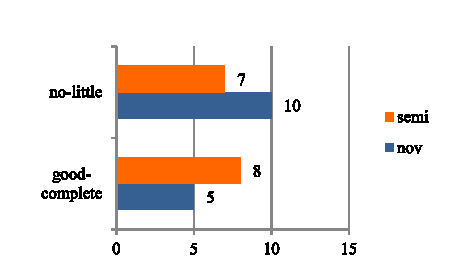
\includegraphics[width=.5\textwidth]{figures/kloster/figure8.pdf}
 \caption{Reading quality of dictionary entries}
 \label{kloster:fig:8}
\end{figure}

\begin{figure}
    \begin{tikzpicture}
        \begin{axis}[
            width  = \textwidth,
            height = .3\textheight,
            ylabel={},
            xlabel={}, 
            symbolic x coords={ICA/mit, ICA/ido, ICA/fic, ICA/fen},
            xtick=data,
            axis lines*=left,  
            ymin=0,
            ybar,
            bar width = 18pt,
            nodes near coords,
            nodes near coords align={vertical},
            axis on top,
            ymajorgrids, tick align=inside,
            major grid style={draw=white},
            enlarge x limits=true, 
        ]    
        \addplot+[lsMidBlue!80!black,fill=lsMidBlue] coordinates {(ICA/mit,1.1) (ICA/ido,1.4) (ICA/fic,1.9) (ICA/fen,0.9)};
        \addplot+[lsMidOrange!80!black,fill=lsMidOrange] coordinates {(ICA/mit,0.7) (ICA/ido,0.8) (ICA/fic,0.9) (ICA/fen,0.8)};
        \legend{nov, semi}
        \end{axis}
    \end{tikzpicture}
    %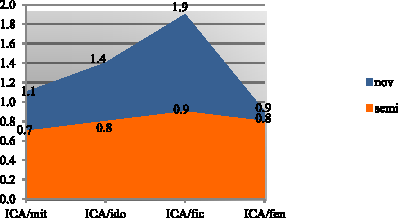
\includegraphics[width=.5\textwidth]{figures/kloster/figure9.pdf}
    \caption{Individual comprehension evaluation}
    \label{kloster:fig:9}
\end{figure}

A number of participants (8 semi-professionals and 5 \isi{novices}) were very thorough in reading the entries in the dictionary. In this context, it is possible to distinguish two types of behavior. The first type reads the dictionary entries word for word from the beginning to the end, fixating certain words longer than others, and returns to the translation after having finished reading. The second type reads the first dictionary entry carefully, then jumps back and forth between the entries, reading and rereading parts of them. 

\newpage 
The monolingual dictionary itself may induce reception difficulties, because its entries contain words which may be unknown to participants. In two cases, semi-professionals went beyond the first entry and looked up words related to the entry itself. Participant P09, looking up the meaning of \textit{idolo:} \textsf{<(...) finds the words 'venerate' in the second contribution, types 'venerato', no solution, types 'venerare', reads the first two lines and goes back to translation>} and participant P11, looking up the meaning of \textit{mito:} \textsf{<(...) clicks on 'mitico', scans the contribution, stops at 'miticamente, in modo m.' then at 'che costituisce,} \textsf{è...} \textsf{leggenda', returns to translation>.} It was expected that both groups would not consult the dictionary for the purpose of comprehension, but rather for other reasons. Although participants were not prompted to comment on the usage of the dictionary, some of them did it voluntarily. According to most verbal reports, the main reason for using the dictionary was either to confirm or to reject the idea in translator's mind. Several participants compared the \ili{German} ``definition'' of \textit{Idol} with the contribution of \textit{idolo} in the monolingual dictionary to see how far they coincide. Participant P09, for example, interpreted the explanation of the word \textit{idolo} in favor of the \ili{German} version \textit{Idol} and decided to use it. 

\subsection{False friends: individual comprehension evaluation} 
Assuming that visual parameters are unconscious indicators of reception, individual comprehension evaluation is the conscious assessment of reception difficulty. The results show (\figref{kloster:fig:9}) that \isi{novices} evaluate the reception difficulty slightly higher than semi-professionals, they do, however, not reach the mark \textit{difficult.} These results are not surprising and are quite in line with the visual parameters. 

\section{Conclusion}

Summarizing the findings and going back to the hypotheses, we cannot confirm that \isi{novices} process false friends in terms of reading and comprehension faster than semi-professionals. A large proportion of \isi{novices} seem to be aware of the treacherous nature of false friends, as the results of the retrospective interview and the product evaluation show. Still, a large number of \isi{novices}, as opposed to semi-professionals (18 to 9), considered false friends a simple task and picked the \isi{cognate} solution, without further reflection. These results confirm that the behavior of non-professionals seems automatic, because they are often completely unaware of potential problems and therefore process relatively little \citep{Jaaskelainen1999}. The very similar amount of visual attention spent on false friends by both groups can also be explained by the fact that semi-professionals spend more time producing the target text and \isi{novices}, instead, are involved in a more time-consuming source text analysis. The \isi{fixation count} data show that novices fixate false friends slightly more frequently than semi-professionals, which demonstrates that they merely reread parts of the source text several times. Semi-professionals, as expected, are for the most part aware of the difficulties associated with the false friends and carefully consider their translation solutions, which results among other things in a choice of creative solutions. These results are in line with the conclusion by \citet{Jonasson1998} that professionals are more aware of potential problems in translation. Furthermore, extensive processing, as the results of the retrospective interviews show, ``is likely to yield better results, for experts and \isi{novices} alike'' \citep[233]{Breedveld2002}, which explains the outcome of the product analysis. 

As for the frequency of dictionary consultations, it became apparent that false friends are not a typical source of reception problems, which would severely impede the understanding of the text. The frequency of lookups is low and nearly identical in both groups. The main purposes of consultations were to confirm or reject the pre-existing idea in a translator's mind, i.e. to compare one's own understanding with the explanation of the dictionary entry.

In terms of \isi{translation competence} development and in particular its bilingual/linguistic proportion, we observe a notable progression from the novice to the \isi{semi-professional} level.  Furthermore, we see that apparently similar behaviour, e.g. similar \isi{total fixation duration}, is motivated differently, as the complementing data show.  

Detailed production data, which is missing in the small framework of the present evaluation, would add further clarity to the processing of the target text.  Further categories of language contrasts (collocations, realia, proper names etc.) will be analysed in the framework of the present study by applying the same methodology and thereby laying the foundations for the comparison of different categories of language contrasts. Translator performance, e.g. related to the use of reference materials, will presumably differ between categories.

{\sloppy
\printbibliography[heading=subbibliography,notkeyword=this]
}
\end{document}


% TODO: Was ist das hier??!
% überprüfe Accents, ...
% \textbf{Robot infermiere: il fenomeno che furoreggia negli ospedali} 
% 
% \begin{styleStandardWeb}
% Ecco che in corsia* entra in scena il robot infermiere, l'idolo dei medici italiani, progettato dall‘Università La Sapienza e finanziato dal Policlinico Gemelli di Roma. C‘è da sorprendersi come si muova da una corsa all‘altra con disinvoltura, dando una mano sia a medici che a pazienti. \`{E} cosi gentile che distribuisce anche merendine e pizze al taglio. 
% \end{styleStandardWeb}
% 
% \begin{styleStandardWeb}
% \`{E} in grado inoltre di sollevare i pazienti dalle sedie a rotelle che hanno un peso massimo di 135 chili!\\
% E** il braccio destro del personale e ha sempre un occhio di riguardo per i pazienti.\\
% ``A volte si pensa di avere a che fare con una persona in carne e ossa! \`{E} semplicemente un mito!`` commentano alcuni.\\
% Questa è la nuova fiction di Rai 1, ``L‘infermiere Roberto``, in onda questa sera dalle 21:00. Non perderne neanche una puntata!\\
% *corsa\\
% **\`{E} 
% \end{styleStandardWeb}
% 
% \begin{styleStandardWeb}
% (http://archiviostorico.corriere.it/1993/gennaio/03/robot\_infermiere\_furoreggia\_negli\_ospedali\_co\_0\_9301032938.shtml) 
% \end{styleStandardWeb}
% 
% \begin{styleStandardWeb}
% \textbf{Non fare orecchie da mercante: leggi qualche libro, farai crescere l‘economia!} 
% \end{styleStandardWeb}
% 
% \begin{styleStandardWeb}
% Ebbene sì: l‘andamento debole del nostro PIL dipende anche dalla scarsa propensione degli italiani a leggere un libro. Ed ecco perché il Ministero dell‘Istruzione proporrà nei prossimi giorni una campagna nazionale apposta per la promozione della lettura.\\
% Dati economici alla mano, forniti dall‘Associazione degli Editori Italiani (AEI), si delinea un quadro scoraggiante: nel 2009 il 68,7\% non ha toccato neppure un libro (un dato da far drizzare i capelli), mentre i cosidetti topi da biblioteca, ovvero coloro che leggono più di quarantotto libri all‘anno, sonoscesi del 3,5\% rispetto all‘anno precedente (2007), in cui ne furono il 12,7\%. 
% \end{styleStandardWeb}
% 
% \begin{styleStandardWeb}
% Cosa c‘entra tutto questo con il PIL? La risposta è sotto gli occhi di tutti: più libri si vendono, meglio è per l‘economia del Paese. ``Occorrono iniziative, perchè il tasso di lettura aumenti``, afferma il direttore dell‘AEI, sostenendo che ``la conoscenza è la forza della produttività. Se non riusiamo* ad aumentarla, saremo spacciati``. *riusciamo 
% \end{styleStandardWeb}
% 
% \begin{styleStandardWeb}
% http://www.ilsole24ore.com/art/notizie/2013-03-20/italiano-legge-neppure-libro-093659.shtml?uuid=AbpOxofH 
% \end{styleStandardWeb}
% 
% \begin{styleStandardWeb}
% \textbf{False friends} 
% \end{styleStandardWeb}
% 
% \begin{styleStandardWeb}
% \textbf{Context} 
% \end{styleStandardWeb}
% 
% \begin{styleStandardWeb}
% fenomeno 
% \end{styleStandardWeb}
% 
% \begin{styleStandardWeb}
% Robot infermiere: il fenomeno che furoreggia negli ospedali 
% \end{styleStandardWeb}
% 
% \begin{styleStandardWeb}
% idolo 
% \end{styleStandardWeb}
% 
% \begin{styleStandardWeb}
% Ecco che in corsia entra in scena il robot infermiere, l‘idolo dei medici italiani, progettato dall‘Università La Sapienza e finanziato dal Policlinico Gemelli di Roma. 
% \end{styleStandardWeb}
% 
% \begin{styleStandardWeb}
% fiction 
% \end{styleStandardWeb}
% 
% \begin{styleStandardWeb}
% Questa è una nuova fiction di Rai 1, ``L‘infermiere Roberto``, in onda questa sera dalle 21:00. Non perderne neanche una puntata! 
% \end{styleStandardWeb}
% 
% \begin{styleStandardWeb}
% mito 
% \end{styleStandardWeb}
% 
% \begin{styleStandardWeb}
% ``A volte si pensa di avere a che fare con una persona in carne e ossa. \`{E} semplicemente un mito!`` commentano alcuni. 
% \end{styleStandardWeb}
% 
% 
% \begin{verbatim}%%move bib entries to  localbibliography.bib



% Taylor, I. (1976) „Similarity between \ili{French} and English Words: a Factor to be Considered in Bilingual Language Behavior?“ Journal of Psycholinguistic Research 5 (1): 85-94.

% Browne, R.L. (1982) Aural and Visual Recognition of Cognates and their Implications for the Teaching of Cognate Languages. Ph.D. Dissertation. Cambridge, MA: Harvard University.

% Perkins, C. (1985) “Sensitizing Advanced Learners to Problems of L1-L2 Translation.” In: Titford, C. and Hieke, A.E. (eds.) Translation in Foreign Language Teaching and Testing. Tübingen: Gunter Narr Verlag, 51-72.

% Levý, J. (1967) “Translation as a Decision Process.” In: To Honor Roman Jakobson II. The Hague: Mouton, 1171-1182.

% PACTE (2000) "Acquiring \isi{translation competence}: hypotheses and methodological problems in a research project."  In: Beeby, A., Ensinger, D. and Presas, M. (eds.)  Investigating Translation: Selected papers from the 4th International Congress on Translation, Barcelona, 1998. Amsterdam/Philadelphia: John Benjamins, 99-106.

% \end{verbatim} 
